\documentclass[12pt,addpoints]{repaso}
\grado{2}
\nivel{Secundaria}
\cicloescolar{2025-2026}
\materia{Matemáticas}
\unidad{1}
\title{Practica la Unidad}
\aprendizajes{
      \item Resuelve problemas que impliquen la suma, resta, la multiplicación y la división de números enteros, aplicando las reglas correspondientes.
      \item Identifica y ubica números negativos en una recta numérica, comparando su magnitud.
      \item Aplica las propiedades de las potencias a números negativos en la resolución de problemas.
      \item Resuelve problemas que involucren las leyes de los exponentes, y expresa números en notación científica.
      \item Resuelve problemas de contexto científico y tecnológico utilizando la notación científica.
      \item Identifica y ubica puntos en el plano cartesiano, y comprende la estructura de los cuadrantes.
      \item Calcula la pendiente de una recta y comprende su significado en diferentes contextos.
      \item Resuelve problemas que involucren el uso de porcentajes, mediante la ``regla de tres''.
}
\author{Melchor Pinto, J.C.}
\begin{document}
\INFO
\begin{multicols}{2}
	\tableofcontents
\end{multicols}
\newpage
\begin{questions}

	\section{Cálculos numéricos}

	\subsection{Suma de números}

	\questionboxed[2]{Realiza las siguientes \emph{sumas}:

		\begin{parts}
			\begin{multicols}{3}
				\part \ifprintanswers{\opadd[hfactor=decimal,resultstyle=\color{red},carryadd=true]{464}{303}}
				\else{\opadd[hfactor=decimal,resultstyle=\color{white},carryadd=false]{464}{303}}\fi

				\part \ifprintanswers{\opadd[hfactor=decimal,resultstyle=\color{red},carryadd=true]{647.94}{564.973}}
				\else{\opadd[hfactor=decimal,resultstyle=\color{white},carryadd=false]{647.94}{564.973}}\fi

				\part \ifprintanswers{\opadd[hfactor=decimal,resultstyle=\color{red},carryadd=true]{98.97}{46.52}}
				\else{\opadd[hfactor=decimal,resultstyle=\color{white},carryadd=false]{98.97}{46.52}}\fi

				\columnbreak%

				\part \ifprintanswers{\opadd[hfactor=decimal,resultstyle=\color{red},carryadd=true]{5423}{3214}}
				\else{\opadd[hfactor=decimal,resultstyle=\color{white},carryadd=false]{5423}{3214}}\fi

				\part \ifprintanswers{\opadd[hfactor=decimal,resultstyle=\color{red},carryadd=true]{344.64}{280.79}}
				\else{\opadd[hfactor=decimal,resultstyle=\color{white},carryadd=false]{344.64}{280.79}}\fi

				\part \ifprintanswers{\opadd[hfactor=decimal,resultstyle=\color{red},carryadd=true]{67.67}{52.97}}
				\else{\opadd[hfactor=decimal,resultstyle=\color{white},carryadd=false]{67.67}{52.973}}\fi

				\columnbreak%

				\part \ifprintanswers{\opadd[hfactor=decimal,resultstyle=\color{red},carryadd=true]{54.54}{19.23}}
				\else{\opadd[hfactor=decimal,resultstyle=\color{white},carryadd=false]{54.54}{19.23}}\fi

				\part $321+51+134=$ \fillin[$506$][0in]

				\part $0.1+0.02+0.03+0.4=$ \fillin[$0.55$][0in]
			\end{multicols}
		\end{parts}
	}

	\subsection{Resta de números}

	\questionboxed[2]{Realiza las siguientes \emph{restas}:

		\begin{parts}
			\begin{multicols}{3}
				\part \ifprintanswers{   \opsub[hfactor=decimal,resultstyle=\color{red},carryadd=true,carrysub=true]{82.48}{28.19} }
				\else{            \opsub[hfactor=decimal,resultstyle=\color{white},carryadd=false,carrysub=false]{82.48}{28.19}}\fi

				\part \ifprintanswers{   \opsub[hfactor=decimal,resultstyle=\color{red},carryadd=true,carrysub=true]{495}{92} }
				\else{            \opsub[hfactor=decimal,resultstyle=\color{white},carryadd=false,carrysub=false]{495}{92}}\fi

				\part \ifprintanswers{   \opsub[hfactor=decimal,resultstyle=\color{red},carryadd=true,carrysub=true]{937}{682} }
				\else{            \opsub[hfactor=decimal,resultstyle=\color{white},carryadd=false,carrysub=false]{937}{682}}\fi

				\part \ifprintanswers{   \opsub[hfactor=decimal,resultstyle=\color{red},carryadd=true,carrysub=true]{341}{212} }
				\else{            \opsub[hfactor=decimal,resultstyle=\color{white},carryadd=false,carrysub=false]{341}{212}}\fi

				\part \ifprintanswers{   \opsub[hfactor=decimal,resultstyle=\color{red},carryadd=true,carrysub=true]{465.76}{292.41} }
				\else{            \opsub[hfactor=decimal,resultstyle=\color{white},carryadd=false,carrysub=false]{465.76}{292.41}}\fi

				\part \ifprintanswers{   \opsub[hfactor=decimal,resultstyle=\color{red},carryadd=true,carrysub=true]{762}{394} }
				\else{            \opsub[hfactor=decimal,resultstyle=\color{white},carryadd=false,carrysub=false]{762}{394}}\fi

				\part \ifprintanswers{   \opsub[hfactor=decimal,resultstyle=\color{red},carryadd=true,carrysub=true]{850}{472} }
				\else{            \opsub[hfactor=decimal,resultstyle=\color{white},carryadd=false,carrysub=false]{850}{472}}\fi

				\part \ifprintanswers{   \opsub[hfactor=decimal,resultstyle=\color{red},carryadd=true,carrysub=true]{945}{173} }
				\else{            \opsub[hfactor=decimal,resultstyle=\color{white},carryadd=false,carrysub=false]{945}{173}}\fi

				\part \ifprintanswers{   \opsub[hfactor=decimal,resultstyle=\color{red},carryadd=true,carrysub=true]{0.1}{0.02} }
				\else{            \opsub[hfactor=decimal,resultstyle=\color{white},carryadd=false,carrysub=false]{0.1}{0.02}}\fi
			\end{multicols}
		\end{parts}
	}

	\subsection{Multiplicación de números}

	\questionboxed[2]{Realiza las siguientes \emph{multiplicaciones}:

		\begin{parts}
			\begin{multicols}{4}
				\part \ifprintanswers{\opmul[hfactor=decimal,resultstyle=\color{red},displayintermediary=None]{284}{31} }
				\else{\opmul[hfactor=decimal,resultstyle=\color{white},displayintermediary=None]{284}{31}}\fi\\[1em]

				\part \ifprintanswers{\opmul[hfactor=decimal,resultstyle=\color{red},displayintermediary=None]{26.37}{13} }
				\else{\opmul[hfactor=decimal,resultstyle=\color{white},displayintermediary=None]{26.37}{13}}\fi\\[1em]

				\part \ifprintanswers{\opmul[hfactor=decimal,resultstyle=\color{red},displayintermediary=None]{411}{4} }
				\else{\opmul[hfactor=decimal,resultstyle=\color{white},displayintermediary=None]{411}{4}}\fi\\[1em]

				\part \ifprintanswers{\opmul[hfactor=decimal,resultstyle=\color{red},displayintermediary=None]{57}{1.39} }
				\else{\opmul[hfactor=decimal,resultstyle=\color{white},displayintermediary=None]{57}{1.39}}\fi\\[1em]

				\part \ifprintanswers{\opmul[hfactor=decimal,resultstyle=\color{red},displayintermediary=None]{24.13}{15} }
				\else{\opmul[hfactor=decimal,resultstyle=\color{white},displayintermediary=None]{24.13}{15}}\fi\\[1em]

				\part \ifprintanswers{\opmul[hfactor=decimal,resultstyle=\color{red},displayintermediary=None]{1851}{21} }
				\else{\opmul[hfactor=decimal,resultstyle=\color{white},displayintermediary=None]{1851}{21}}\fi\\[1em]

				\part \ifprintanswers{\opmul[hfactor=decimal,resultstyle=\color{red},displayintermediary=None]{515}{37} }
				\else{\opmul[hfactor=decimal,resultstyle=\color{white},displayintermediary=None]{515}{37}}\fi\\[1em]

				\part \ifprintanswers{\opmul[hfactor=decimal,resultstyle=\color{red},displayintermediary=None]{225}{9} }
				\else{\opmul[hfactor=decimal,resultstyle=\color{white},displayintermediary=None]{225}{9}}\fi\\[1em]
			\end{multicols}
		\end{parts}
	}

	\subsection{División de números}

	\questionboxed[2]{Calcula el \textbf{cociente} y el \textbf{residuo} de las siguientes \emph{divisiones}:

		\begin{parts}
			\begin{multicols}{3}
				\part $785 \divisionsymbol 125=$ \\[1em]
				Cociente: \fillin[6][0in]\\
				Residuo: \fillin[35][0in]\\

				\part $655.23 \divisionsymbol 23=$ \\[1em]
				Cociente: \fillin[28][0in]\\
				Residuo: \fillin[11][0in]\\

				\part $123 \divisionsymbol 1.2=$ \\[1em]
				Cociente: \fillin[102][0in] \\
				Residuo: \fillin[6][0in]\\

				\part $723 \divisionsymbol 8=$ \\[1em]
				Cociente: \fillin[90][0in]\\
				Residuo: \fillin[3][0in]\\

				\part $90 \divisionsymbol 21=$ \\[1em]
				Cociente: \fillin[4][0in]\\
				Residuo: \fillin[6][0in]\\

				\part $22 \divisionsymbol 0.2=$ \\[1em]
				Cociente: \fillin[110][0in]\\
				Residuo: \fillin[0][0in]\\
			\end{multicols}
		\end{parts}
	}

	\subsection{Resolución de problemas}

	\questionboxed[2]{Resuelve los siguientes problemas:

		\begin{parts}
			\begin{multicols}{2}
				\part Una computadora tiene un disco duro de 368 GB de memoria, si varios programas ocupan 128.75 GB. ¿Qué cantidad de memoria está libre?

				\begin{solutionbox}{1.2cm}
					$368-128.75=$ \fillin[$239.25$][0in]
				\end{solutionbox}

				\part En un estacionamiento conté 57 automóviles, 31 camionetas y 23 taxis, ¿cuántos vehículos había en total?

				\begin{solutionbox}{1.2cm}
					$57+31+23=$ \fillin[$111$][0in]
				\end{solutionbox}

				\part El precio de 385 artículos comerciales es de 1232 pesos. ¿Cuál es el precio unitario de cada artículo?

				\begin{solutionbox}{1.2cm}
					$1232 \divisionsymbol 385=$ \fillin[$3.20$][0in]
				\end{solutionbox}
				
				\part Las ventas de boletos que registra un cine en un fin de semana son las siguientes: 490 boletos vendidos el viernes, 780 el sábado y 1234 el domingo. ¿Cuántos boletos se vendieron en total?
				
				\begin{solutionbox}{1.2cm}
					$490+780+1234=$ \fillin[$2504$][0in]
				\end{solutionbox}

				\part Una pintura tiene un costo de 25.75 pesos el litro, una persona compra 48 litros. ¿Cuánto debe pagar?
			
				\begin{solutionbox}{1.2cm}
					$25.75 \times 48=$ \fillin[$1236$][0in]
				\end{solutionbox}
			
				\part Un elástico se estira tres veces su longitud en su estado normal. Si mide 5.23 cm en su estado normal, ¿cuántos centímetros alcanza al ser estirado?
			
				\begin{solutionbox}{1.2cm}
					$5.23 \times 3=$ \fillin[$15.69$][0in]
				\end{solutionbox}

				\part Si un dólar equivale a 19 pesos. ¿Cuántos pesos equivaldrán 615 dólares?
			
				\begin{solutionbox}{1.2cm}
					$19 \times 615=$ \fillin[$11685$][0in]
				\end{solutionbox}

				\part En un recipiente con agua, se agregaron otros 12.56 litros,llegando a completar 15.89 litros de agua. ¿Cuántos litros de agua había inicialmente en el recipiente?
			
				\begin{solutionbox}{1.2cm}
					$15.89 \times 12.56=$ \fillin[$3.33$][0in]
				\end{solutionbox}
			\end{multicols}
		\end{parts}
	}

	\section{Números negativos}

	\subsection{Ubicación en la recta numérica}

	\questionboxed[2]{Escribe el \textbf{número} que representa el punto indicado en la recta numérica de cada uno de los siguientes incisos.

		\begin{multicols}{2}
			\begin{parts}

				\part 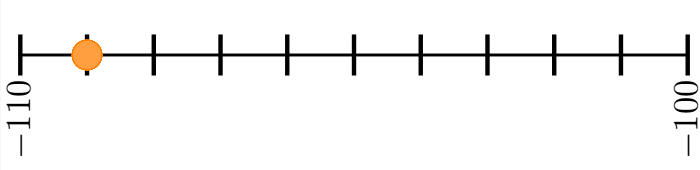
\includegraphics[width=0.8\linewidth]{../images/recta_num_-109.png} \\[-0.5em]    \qquad \fillin[$-109$][0in]

				\part 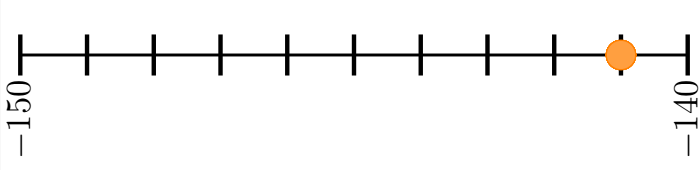
\includegraphics[width=0.8\linewidth]{../images/recta_num_-141.png} \\[-0.5em]    \qquad \fillin[$-141$][0in]

				\part 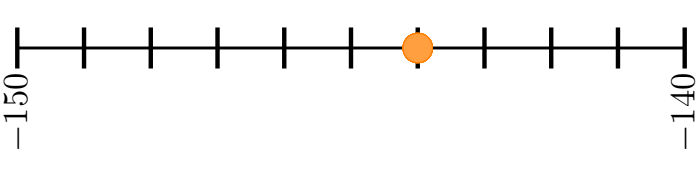
\includegraphics[width=0.8\linewidth]{../images/recta_num_-144.png}   \\[-0.5em]  \qquad \fillin[$-144$][0in]

				\part 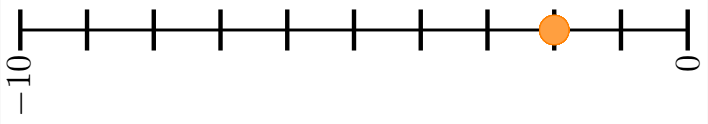
\includegraphics[width=0.8\linewidth]{../images/recta_num_-2.png} \\[-0.5em]  \qquad   \fillin[$-2$][0in]

				\part 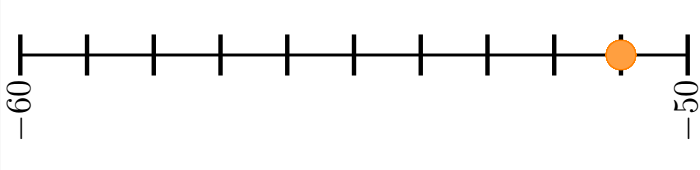
\includegraphics[width=0.8\linewidth]{../images/recta_num_-51.png}   \\[-0.5em] \qquad  \fillin[$-51$][0in]

				\columnbreak%


				\part 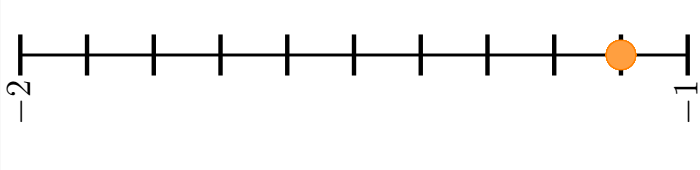
\includegraphics[width=0.8\linewidth]{../images/recta_num_-1.1.png}\\[-0.5em]   \qquad \fillin[$-1.1$][0in]

				\part 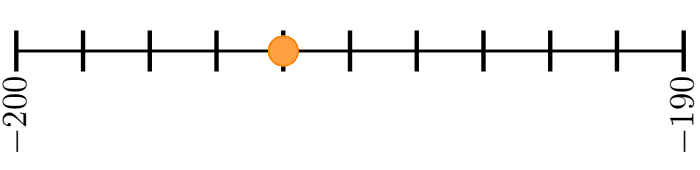
\includegraphics[width=0.8\linewidth]{../images/recta_num_-196.png}  \\[-0.5em]   \qquad \fillin[$-196$][0in]

				\part 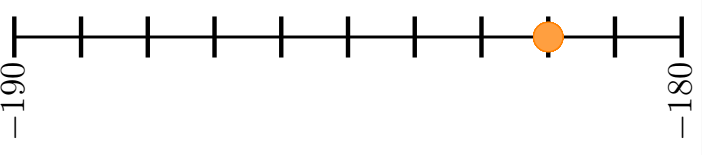
\includegraphics[width=0.8\linewidth]{../images/recta_num_-182.png}  \\[-0.5em]   \qquad \fillin[$-182$][0in]

				\part 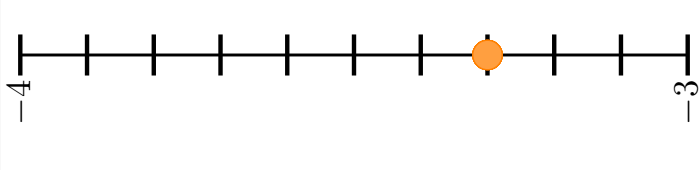
\includegraphics[width=0.8\linewidth]{../images/recta_num_-3.3.png}\\[-0.5em]   \qquad \fillin[$-3.3$][0in]

				\part 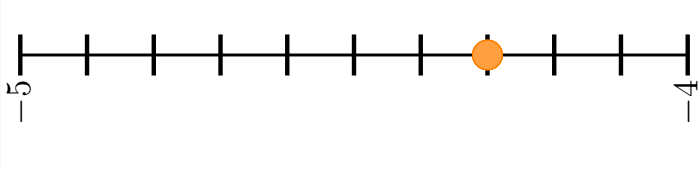
\includegraphics[width=0.8\linewidth]{../images/recta_num_-4.3.png}  \\[-0.5em]   \qquad \fillin[$-4.3$][0in]
			\end{parts}
		\end{multicols}
	}


	% \addcontentsline{toc}{subsection}{Comparación de negativos}
	\subsection{Comparación de negativos}

	\questionboxed[2]{Escribe sobre la línea el símbolo de mayor que ($>$), menor que ($<$), o igual ($=$) según corresponda.

		\begin{multicols}{3}
			\begin{parts}
				\part $-2$ \fillin[$>$][0.5in] $-5$\\[0.25em]
				\part $-27$ \fillin[$<$][0.5in] $-22$\\[0.25em]
				\part $-75$ \fillin[$<$][0.5in] $-70$\\[0.25em]
				\part $-15.2$ \fillin[$>$][0.5in] $-16$\\[0.25em]
				\part $-1$ \fillin[$>$][0.5in] $-4$\\[0.25em]
				\part $-28.9$ \fillin[$<$][0.5in] $-28.2$\\[0.25em]
				\part $-110$ \fillin[$<$][0.5in] $-108$\\[0.25em]
				\part $-5.8$ \fillin[$<$][0.5in] $-5.5$\\[0.25em]
				\part $-10$ \fillin[$<$][0.5in] $-2$\\[0.25em]
				\part $-105$ \fillin[$>$][0.5in] $-150$\\[0.25em]
				\part $-10$ \fillin[$>$][0.5in] $-12$\\[0.25em]
				\part $-29$ \fillin[$>$][0.5in] $-30$\\[0.25em]
			\end{parts}
		\end{multicols}
	}



	% \addcontentsline{toc}{subsection}{Suma y resta con negativos}
	\subsection{Suma y resta con negativos}

	\questionboxed[4]{Realiza las siguientes sumas y restas con números negativos:

		\begin{multicols}{3}
			\begin{parts}
				\part $(14)+(-9)=$ \fillin[$5$][0in]

				\part $101-116=$ \fillin[$-15$][0in]

				\part $80-100=$ \fillin[$-20$][0in]

				\part $12-20=$ \fillin[$-8$][0in]

				\part $-47+35=$ \fillin[$-12$][0in]

				\part $55-99=$ \fillin[$-44$][0in]

				\part $(16)-(-20)+(39)=$ \fillin[$75$][0in]

				\part $-17-17=$ \fillin[$-34$][0in]

				\part $33-29=$ \fillin[$4$][0in]

				 \part $-223+67=$ \fillin[$-156$][0in]

				 \part $(56)-(-24)=$ \fillin[$80$][0in]

				\part $-(-25)+(-24)=$ \fillin[$1$][0in]

				\part $-235+304=$ \fillin[$69$][0in]

				\part $198-189=$ \fillin[$9$][0in]

				\part $-201.1-9.4=$ \fillin[$-210.5$][0in]

				\part $201.1-9.4=$ \fillin[$191.7$][0in]

				\part $-201.1+9.4=$ \fillin[$-191.7$][0in]

			\end{parts}
		\end{multicols}
	}


	% \addcontentsline{toc}{subsection}{Multiplicación y división con negativos}
	\subsection{Multiplicación y división con negativos}

	\questionboxed[4]{Realiza las siguientes multiplicaciones y divisiones con números negativos:

		\begin{multicols}{2}
			\begin{parts}
				\part $(-16)\divisionsymbol (-8)=$ \fillin[$-\dfrac{1}{2}$][0in]

				\part $(15)(-4)=$ \fillin[$-60$][0in]

				\part $(-80)\divisionsymbol (20)=$ \fillin[$-4$][0in]

				\part $(66)\divisionsymbol (-33)\divisionsymbol (-2)\divisionsymbol (10)=$ \fillin[$\dfrac{1}{10}$][0in]

				\part $(31)\divisionsymbol (-62)=$ \fillin[$-\dfrac{1}{2}$][0in]

				\part $(-18)(-25)=$ \fillin[$450$][0in]

				\part $(-4)\divisionsymbol (5)\divisionsymbol (-1)=$ \fillin[$20$][0in]

				\part $(-7)(20)=$ \fillin[$-140$][0in]

				\part $(60)\divisionsymbol (-2)\divisionsymbol (-10)=$ \fillin[$-3$][0in]

				\part $(-11)\divisionsymbol (9)=$ \fillin[$-\dfrac{11}{9}$][0in]

				\part $(-11)(-6)(2)(-3)=$ \fillin[$-396$][0in]

				\part $(25) \divisionsymbol (-3) \divisionsymbol (-5) \divisionsymbol(-10)=$ \fillin[$-\dfrac{1}{6}$][0in]

				\part $(-6)(-6)(-6)=$ \fillin[$-216$][0in]

				\part $(-220)\divisionsymbol (0.2)=$ \fillin[$-1100$][0in]
			\end{parts}
		\end{multicols}
	}


	% \addcontentsline{toc}{subsection}{Potencias con números negativos}
	\subsection{Potencias con números negativos}

	\questionboxed[4]{Realiza las siguientes potencias de números negativos:

		\begin{multicols}{3}
			\begin{parts}
				\part $-2^{9}=$ \fillin[$-512$][0in] \\[-0.5em]
				\part $-1^{80}=$ \fillin[$-1$][0in] \\[-0.5em]
				\part $(-5)^3=$ \fillin[$-125$][0in] \\[-0.5em]
				\part $-5^4=$ \fillin[$-625$][0in] \\[-0.5em]
				\part $(-1)^{75}=$ \fillin[$-1$][0in] \\[-0.5em]
				\part $(-3)^4=$ \fillin[$81$][0in] \\[-0.5em]
				\part $(-10)^3=$ \fillin[$-1000$][0in] \\[-0.5em]
				\part $-10^4=$ \fillin[$-10000$][0in] \\[-0.5em]
				\part $-(-2)^4=$ \fillin[$-16$][0in] \\[-0.5em]
				\part $-(-6)^3=$ \fillin[$216$][0in] \\[-0.5em]
				\part $(-6)^3=$ \fillin[$-216$][0in] \\[-0.5em]
				\part $-6^3=$ \fillin[$-216$][0in] \\[-0.5em]
				\part $(-2)^{10}=$ \fillin[$1024$][0in] \\[-0.5em]
				\part $-(-2)^9=$ \fillin[$512$][0in] \\[-0.5em]
				\part $(-2)^9=$ \fillin[$-512$][0in] \\[-0.5em]
			\end{parts}
		\end{multicols}
	}

	% \addcontentsline{toc}{section}{Exponentes y notación científica}
	\section{Exponentes y notación científica}

	\subsection{Suma de exponentes}

	\questionboxed[4]{Realiza las siguientes operaciones con exponentes:

		\begin{multicols}{3}
			\begin{parts}
				\part $(-5a^4)(-3a^2)=$ \fillin[$15a^6$][0in]

				% \begin{solutionbox}{1cm}
				% 	$(-5a^4)(-3a^2) = 15a^6$
				% \end{solutionbox}

				\part $(5x^3)(-x^{11})=$ \fillin[$-5x^{14}$][0in]

				% \begin{solutionbox}{1cm}
				% 	$(5x^3)(-x^{11})= -5x^{14}$
				% \end{solutionbox}

				\part $x^4x^{12}x^7=$ \fillin[$x^{23}$][0in]


				% \begin{solutionbox}{1cm}
				% 	$x^4x^{12}x^7= x^{23}$
				% \end{solutionbox}

				\part $(-2a^3)(-a)=$ \fillin[$-2a^4$][0in]

				% \begin{solutionbox}{1cm}
				% 	$(-2a^3)(-a)= -2a^4$
				% \end{solutionbox}

				\part $(5y^5)(7y^4)=$  \fillin[$35y^9$][0in]

				% \begin{solutionbox}{1cm}
				% 	$(5y^5)(7y^4)=35y^9$
				% \end{solutionbox}

				\part $(-3a^4)(8a^2)=$ \fillin[$-24a^6$][0in]

				% \begin{solutionbox}{1cm}
					% $(-3a^4)(8a^2) = -24a^6$
				% \end{solutionbox}

				\part $4x^2\cdot x^5\cdot 5x^8=$ \fillin[$20x^{15}$][0in]

				% \begin{solutionbox}{1cm}
				% 	$4x^2\cdot x^5\cdot 5x^8 = 20x^{15}$
				% \end{solutionbox}

				\part $x^2y^3z^4 \cdot x^5z^4=$ \fillin[$x^7y^3z^8$][0in]

				% \begin{solutionbox}{1cm}
				% 	$x^2y^3z^4 \cdot x^5z^4 = x^7y^3z^8$
				% \end{solutionbox}

				\part $7x^2\cdot 3x^4 \cdot 6x^2=$  \fillin[$126x^8$][0in]

				% \begin{solutionbox}{1cm}
				% 	$7x^2\cdot 3x^4 \cdot 6x^2 = 126x^8$
				% \end{solutionbox}
			\end{parts}
		\end{multicols}
	}

	\subsection{Resta de exponentes}

	\questionboxed[3]{Realiza las siguientes operaciones con exponentes:

		\begin{multicols}{3}
			\begin{parts}
				\part $\dfrac{18x^{15}}{6x^{12}}=$ \fillin[$3x^3$][0in]

				% \begin{solutionbox}{1.5cm}
				% 	$\dfrac{18x^{15}}{6x^{12}}=3x^3$
				% \end{solutionbox}

				\part $\dfrac{6x^{7}}{2x^{2}}=$ \fillin[$3x^5$][0in]

				% \begin{solutionbox}{1.5cm}
				% 	$\dfrac{6x^{7}}{2x^{2}}=3x^5$
				% \end{solutionbox}

				\part $\dfrac{a^3b^{9}c^5}{a^2b^{5}c^4}=$ \fillin[$ab^4c$][0in]

				% \begin{solutionbox}{1.5cm}
				% 	$\dfrac{a^3b^{9}c^5}{a^2b^{5}c^4}=ab^4c$
				% \end{solutionbox}

				\part $\dfrac{x^{13}y^{18}z^{4}}{x^{11}y^{9}z^{4}}=$ \fillin[$x^2y^9$][0in]

				% \begin{solutionbox}{1.5cm}
				% 	$\dfrac{x^{13}y^{18}z^{4}}{x^{11}y^{9}z^{4}} = x^2y^9$
				% \end{solutionbox}

				\part $\dfrac{21x^{23}}{7x^{11}}=$ \fillin[$3x^{12}$][0in]

				% \begin{solutionbox}{1.5cm}
				% 	$\dfrac{21x^{23}}{7x^{11}}=3x^{12}$
				% \end{solutionbox}

				\part $\dfrac{25x^{8}}{5x^{3}}=$ \fillin[$5x^5$][0in]

				% \begin{solutionbox}{1.5cm}
				% 	 $\dfrac{25x^{8}}{5x^{3}}=5x^5$
				% \end{solutionbox}

				\part $\dfrac{x^{3}y^{12}z^{13}}{x^{3}y^{12}z^{13}}=$ \fillin[$1$][0in]

				% \begin{solutionbox}{1.5cm}
				% 	$\dfrac{x^{3}y^{12}z^{13}}{x^{3}y^{12}z^{13}} = 1$
				% \end{solutionbox}

				\part $\dfrac{81a^5b^{12}c^9}{9a^3b^{7}c^5}=$ \fillin[$9a^2b^5c^4$][0in]

				% \begin{solutionbox}{1.5cm}
				% 	$\dfrac{81a^5b^{12}c^9}{9a^3b^{7}c^5} = 9a^2b^5c^4$
				% \end{solutionbox}

				\part $\dfrac{5x^{8}}{25x^{3}}=$ \fillin[$\dfrac{x^5}{5}$][0in]

				% \begin{solutionbox}{1.5cm}
				% 	$\dfrac{5x^{8}}{25x^{3}}=\dfrac{x^5}{5}$
				% \end{solutionbox}
			\end{parts}
		\end{multicols}
	}	

	\subsection{Multiplicación de exponentes}

	\questionboxed[4]{Realiza las siguientes operaciones con exponentes:

	\begin{multicols}{3}
		\begin{parts}
			\part $(a^3b^2c^4)^3=$ \fillin[$a^9b^6c^{12}$][0in]

			% \begin{solutionbox}{1cm}
			% 	$(a^3b^2c^4)^3 = a^9b^6c^{12}$
			% \end{solutionbox}
			\part $(x^9y^5z^2)^5=$ \fillin[$x^{45}y^{25}z^{10}$][0in]

			\part $(a^4b^5)^4=$ \fillin[$a^{16}b^{20}$][0in]

			\part $\left(x^9 y^5\right)^{11}=$  \fillin[$x^{99}y^{55}$][0in]

			\part $\left(x^4 y^5\right)^6=$  \fillin[$x^{24}y^{30}$][0in]

			% \begin{solutionbox}{1cm}
			% 	$\left(x^4 y^5\right)^6 = x^{24}y^{30}$
			% \end{solutionbox}

			\part $(x^7y^8z^4w^5)^6=$ \fillin[$x^{42}y^{48}z^{24}w^{30}$][0in]

			\part $(a^3b^7c^5d^4)^4=$ \fillin[$a^{12}b^{28}c^{20}d^{16}$][0in]

			\part $\left(a^3 b^5 c^{11} \right)^7=$  \fillin[$a^{21}b^{35}c^{77}$][0in]

			% \begin{solutionbox}{1cm}
			% 	$\left(a^3 b^5 c^{11} \right)^7 = a^{21}b^{35}c^{77}$
			% \end{solutionbox}

			\part $(a^4b^4c^5d^{11})^5=$ \fillin[$a^{20}b^{20}c^{25}d^{55}$][0in]

		\end{parts}
	\end{multicols}
}	

	\subsection{Notación científica}

	\questionboxed[4]{Escribe en notación científica los siguientes números:

		\begin{multicols}{3}
			\begin{parts}
				\part $55000=$ \fillin[$5.5 \times 10^4$][0in]

				\part $0.00000000024=$ \fillin[$2.4 \times 10^{-10}$][0in]

				\part $101=$ \fillin[$1.01 \times 10^2$][0in]

				\part $750000000000=$ \fillin[$7.5 \times 10^{11}$][0in]

				\part $0.000000015=$ \fillin[$1.5 \times 10^{-7}$][0in]

				\part $900000000000=$ \fillin[$9 \times 10^{11}$][0in]
				 
				\part $80000000=$ \fillin[$8 \times 10^7$][0in]

				\part $0.003=$ \fillin[$3 \times 10^{-3}$][0in]

				\part $0.0000204=$ \fillin[$2.04 \times 10^{-5}$][0in]

				\part $0.000000099=$ \fillin[$9.9 \times 10^{-9}$][0in]

				\part $606000000=$ \fillin[$6.06 \times 10^{8}$][0in]

				\part $10210000000=$ \fillin[$1.021 \times 10^{10}$][0in]

			\end{parts}
		\end{multicols}
	}

	\questionboxed[4]{Escribe en notación decimal los siguientes números:

		\begin{multicols}{4}
			\begin{parts}
				\part $1.2 \times 10^3=$ \fillin[$1200$][0in]

				\part $2.3 \times 10^2=$ \fillin[$230$][0in]

				\part $4 \times 10^{-3}=$ \fillin[$0.004$][0in]

				\part $7 \times 10^{-6}=$ \fillin[$0.000007$][0in]

				\part $2 \times 10^5=$ \fillin[$200000$][0in]

				\part $-3 \times 10^{-2}=$ \fillin[$-0.03$][0in]

				\part $9 \times 10^{0}=$ \fillin[$9$][0in]

				\part $6.3 \times 10^{-3}=$ \fillin[$0.0063$][0in]

				\part $1.2 \times 10^{-1}=$ \fillin[$0.12$][0in]

				\part $80.3 \times 10^{-2}=$ \fillin[$0.803$][0in]

				\part $3 \times 10^{-3}=$ \fillin[$0.003$][0in]

				\part $3 \times 10^{8}=$ \fillin[$300000000$][0in]

			\end{parts}
		\end{multicols}
	}

	\section{Plano cartesiano y la recta}

	\subsection{Ubicación en el plano cartesiano}

	\questionboxed[3]{Escribe las coordenadas de los puntos indicados en el plano cartesiano de cada uno de los siguientes incisos.

		\begin{multicols}{2}
			\begin{parts}
				\part Coordenadas del punto A: \fillin[$(1,5)$][0in]

				\part Coordenadas del punto B: \fillin[$(-3,6)$][0in]

				\part Coordenadas del punto C: \fillin[$(5,-3)$][0in]

				\part Coordenadas del punto D: \fillin[$(-5,0)$][0in]

				\part Coordenadas del punto E: \fillin[$(0,-7)$][0in]

				\part El punto C está en el cuadrante: \fillin[IV][0in]

				\part El punto B está en el cuadrante: \fillin[II][0in]

				\part El punto A está en el cuadrante: \fillin[I][0in]
			\end{parts}
			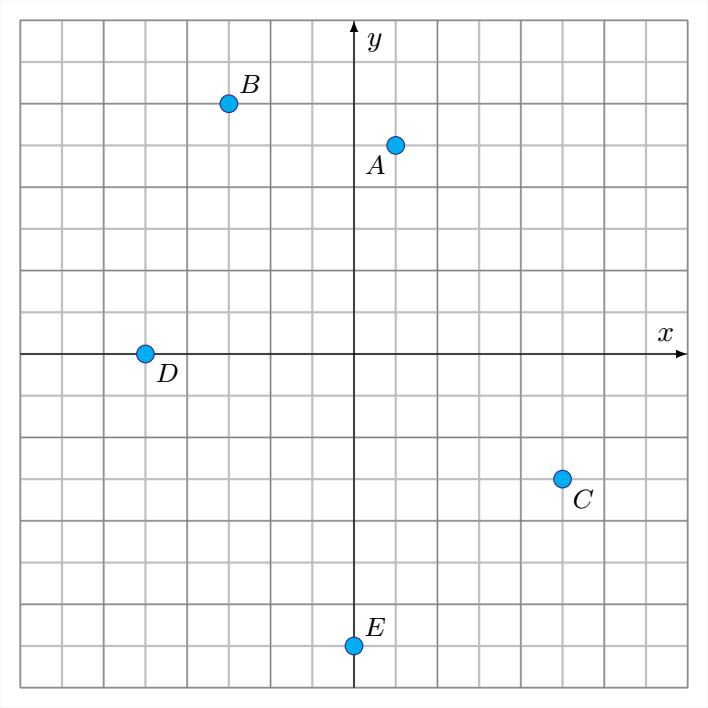
\includegraphics[width=0.75\linewidth]{../images/plano_cart02.png}
		\end{multicols}
	}


	\questionboxed[3]{Escribe las coordenadas de los puntos indicados en el plano cartesiano de cada uno de los siguientes incisos.

		\begin{multicols}{2}
			\begin{parts}
				\part Coordenadas del punto A: \fillin[$(1,4)$][0in]

				\part Coordenadas del punto B: \fillin[$(3,3)$][0in]

				\part Coordenadas del punto C: \fillin[$(-3,1)$][0in]

				\part Coordenadas del punto D: \fillin[$(3,0)$][0in]

				\part Coordenadas del punto E: \fillin[$(0,-1)$][0in]

				\part El punto A está en el cuadrante: \fillin[I][0in]

				\part El punto B está en el cuadrante: \fillin[I][0in]

				\part El punto C está en el cuadrante: \fillin[II][0in]
			\end{parts}
			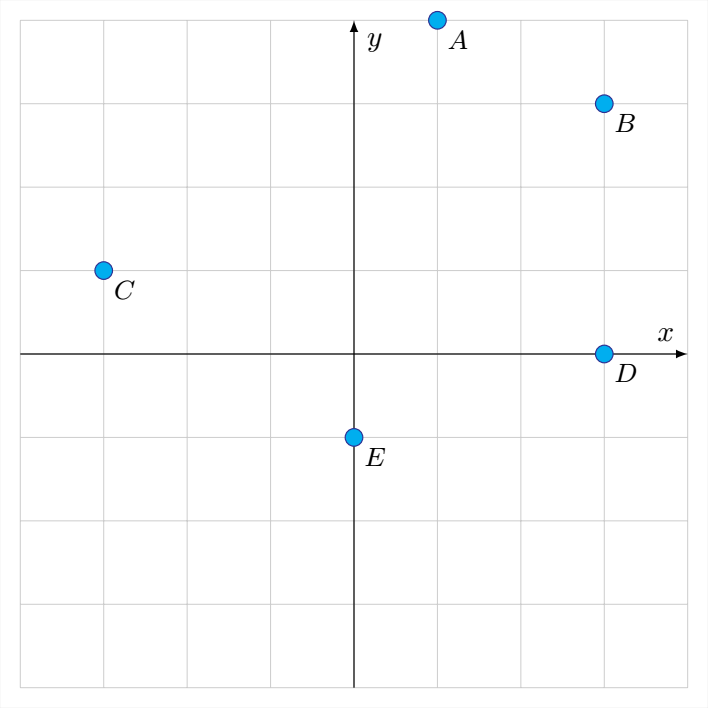
\includegraphics[width=0.75\linewidth]{../images/plano_cart03.png}
		\end{multicols}
	}

	\questionboxed[3]{Escribe las coordenadas de los puntos indicados en el plano cartesiano de cada uno de los siguientes incisos.

		\begin{multicols}{2}
			\begin{parts}
				\part Coordenadas del punto A: \fillin[$(0,1)$][0in]

				\part Coordenadas del punto B: \fillin[$(3,-4)$][0in]

				\part Coordenadas del punto C: \fillin[$(2,-3)$][0in]

				\part Coordenadas del punto D: \fillin[$(0,0)$][0in]

				\part Coordenadas del punto E: \fillin[$(0,-3)$][0in]

				\part El punto B está en el cuadrante: \fillin[IV][0in]

				\part El punto C está en el cuadrante: \fillin[IV][0in]
			\end{parts}
			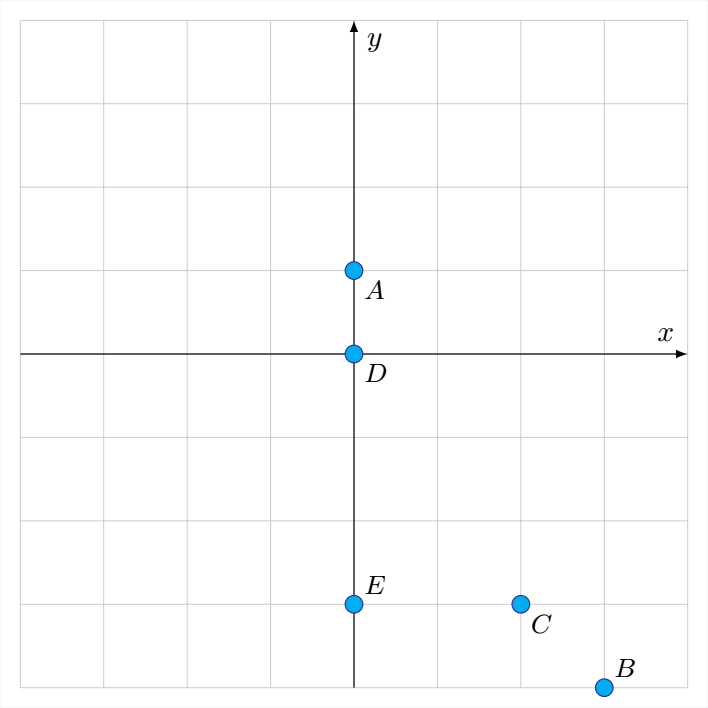
\includegraphics[width=0.75\linewidth]{../images/plano_cart01.png}
		\end{multicols}
	}

	\subsection{Pendiente de una recta}

	\questionboxed[8]{Selecciona la opcion que corresponde a la pendiente de la recta en cada uno de los siguientes incisos:

		\begin{multicols}{2}
			\begin{parts}
				\part
				\begin{minipage}{0.6\linewidth}
					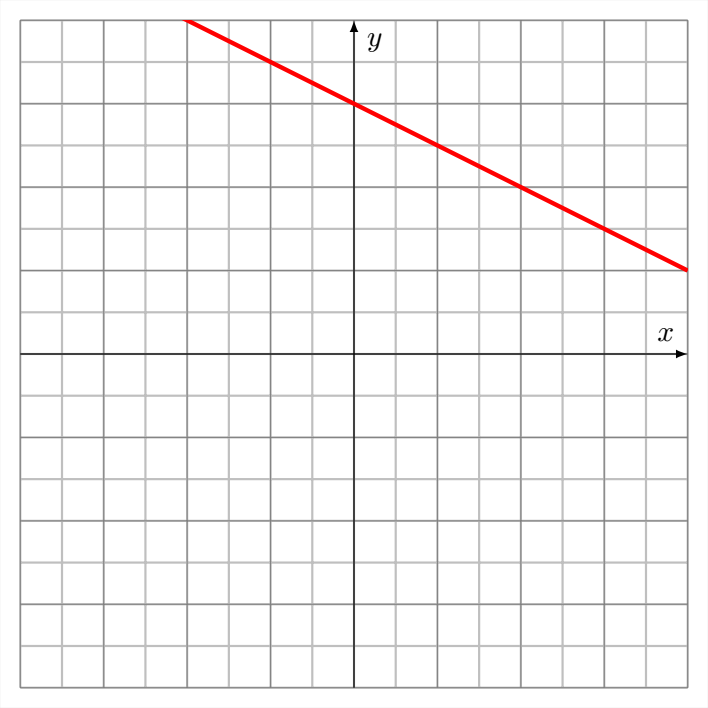
\includegraphics[width=0.8\linewidth]{../images/plano_cart_rect_-1|2x+4.png}
				\end{minipage}%
				\begin{minipage}{0.5\linewidth}
					\begin{choices}
						\choice Positiva
						\CorrectChoice Negativa
						\choice Cero
						\choice Indefinida
					\end{choices}
				\end{minipage}

				\part
				\begin{minipage}{0.6\linewidth}
					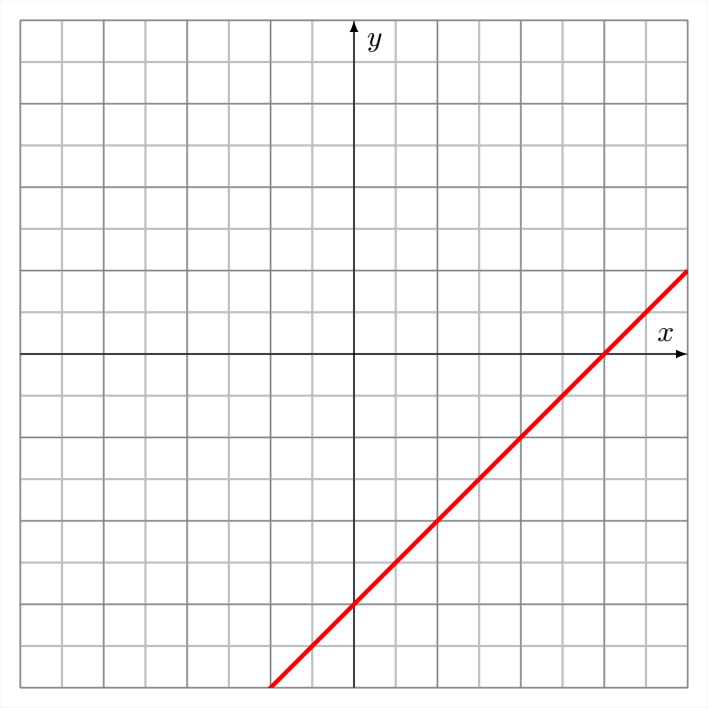
\includegraphics[width=0.8\linewidth]{../images/plano_cart_rect_x-6.png}
				\end{minipage}%
				\begin{minipage}{0.5\linewidth}
					\begin{choices}
						\CorrectChoice Positiva
						\choice Negativa
						\choice Cero
						\choice Indefinida
					\end{choices}
				\end{minipage}

				\part
				\begin{minipage}{0.6\linewidth}
					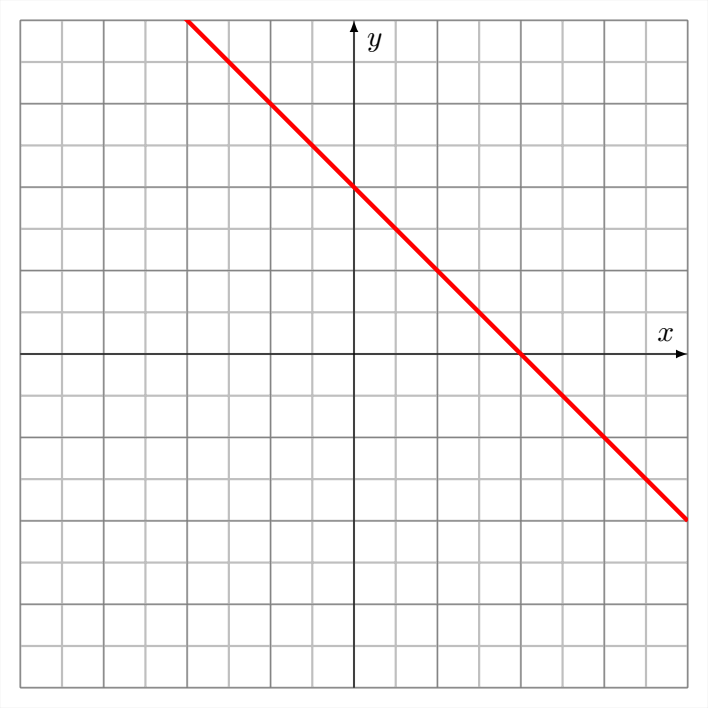
\includegraphics[width=0.8\linewidth]{../images/plano_cart_rect_-x+4.png}
				\end{minipage}%
				\begin{minipage}{0.5\linewidth}
					\begin{choices}
						\choice Positiva
						\CorrectChoice Negativa
						\choice Cero
						\choice Indefinida
					\end{choices}
				\end{minipage}
				
				
				\part
				\begin{minipage}{0.6\linewidth}
					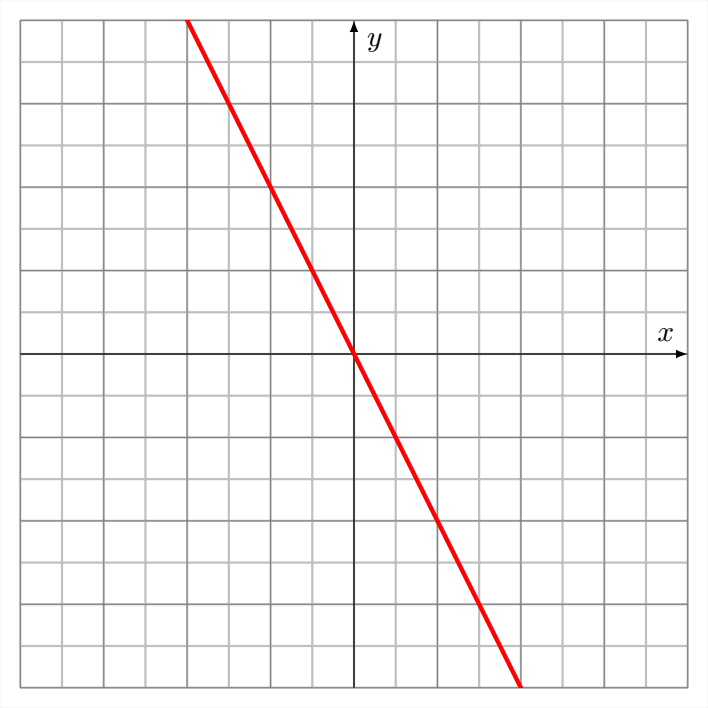
\includegraphics[width=0.8\linewidth]{../images/plano_cart_rect_-2x.png}
				\end{minipage}%
				\begin{minipage}{0.5\linewidth}
					\begin{choices}
						\choice Positiva
						\CorrectChoice Negativa
						\choice Cero
						\choice Indefinida
					\end{choices}
				\end{minipage}

				\part
				\begin{minipage}{0.6\linewidth}
					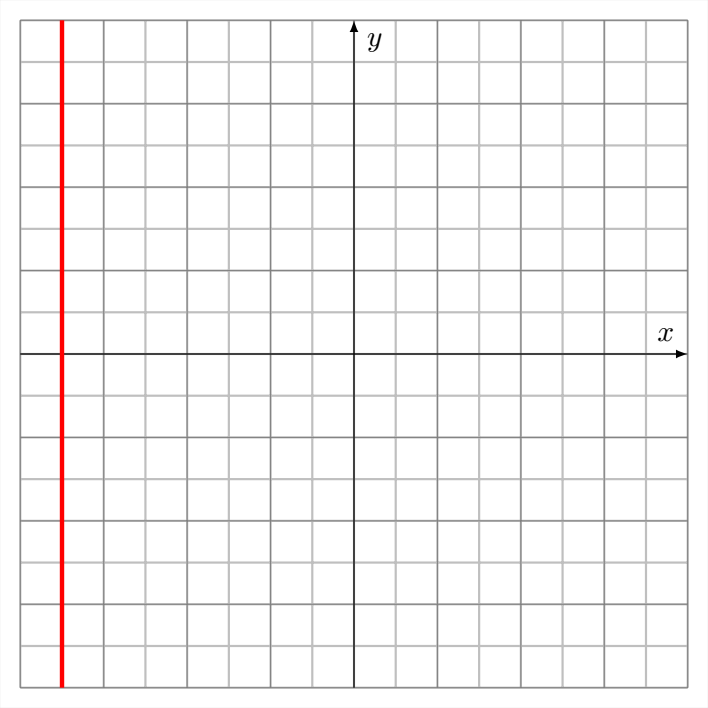
\includegraphics[width=0.8\linewidth]{../images/plano_cart_rect_inf.png}
				\end{minipage}%
				\begin{minipage}{0.5\linewidth}
					\begin{choices}
						\choice Positiva
						\choice Negativa
						\choice Cero
						\CorrectChoice Indefinida
					\end{choices}
				\end{minipage}

				\part
				\begin{minipage}{0.6\linewidth}
					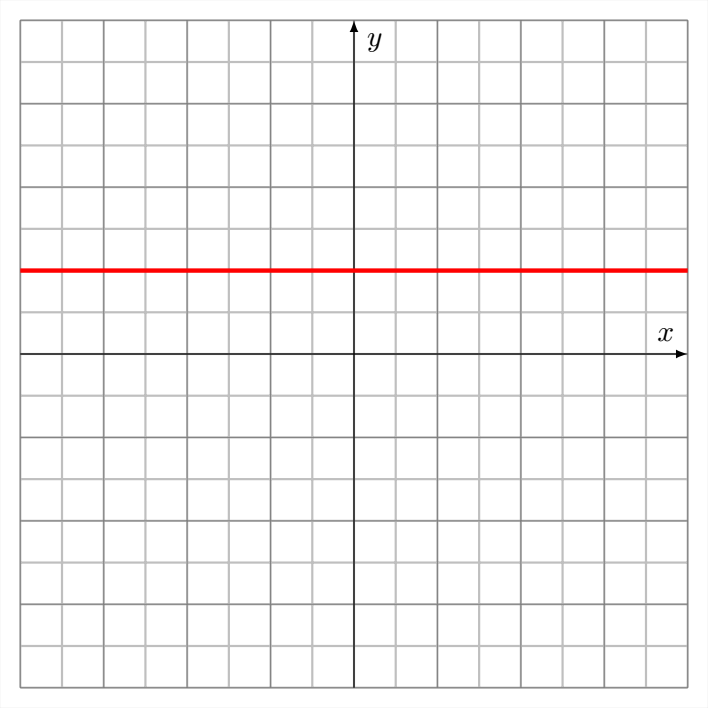
\includegraphics[width=0.8\linewidth]{../images/plano_cart_rect_0.png}
				\end{minipage}%
				\begin{minipage}{0.5\linewidth}
					\begin{choices}
						\choice Positiva
						\choice Negativa
						\CorrectChoice Cero
						\choice Indefinida
					\end{choices}
				\end{minipage}
			\end{parts}
		\end{multicols}
	}


	% \addcontentsline{toc}{subsection}{Pendiente y ordenada}
	\subsection{Pendiente y ordenada}

	\questionboxed[10]{Identifica la pendiente y ordenada de las siguientes rectas:

		\begin{multicols}{3}
			\begin{parts}
				\part $y=-2x$ \\[1em]
				Pendiente = \fillin[$-2$][0in]\\[0.5em]
				Ordenada = \fillin[$0$][0in]

				\part $y=-\dfrac{2}{3}x-5$ \\[1em]
				Pendiente = \fillin[$-\dfrac{2}{3}$][0in]\\[0.5em]
				Ordenada = \fillin[$-5$][0in]

				\part $y=3x+2$ \\[1em]
				Pendiente = \fillin[$3$][0in]\\[0.5em]
				Ordenada = \fillin[$2$][0in]

				\part $y=\dfrac{1}{2}x-3$ \\[1em]
				Pendiente = \fillin[$\dfrac{1}{2}$][0in]\\[0.5em]
				Ordenada = \fillin[$-3$][0in]

				\part $y=-\dfrac{1}{2}x+3$ \\[1em]
				Pendiente = \fillin[$-\dfrac{1}{2}$][0in]\\[0.5em]
				Ordenada = \fillin[$3$][0in]

				\part $y=-3x+3$ \\[1em]
				Pendiente = \fillin[$-3$][0in]\\[0.5em]
				Ordenada = \fillin[$3$][0in]
			\end{parts}
		\end{multicols}
	}


	% \addcontentsline{toc}{subsection}{Ecuación de una recta}
	\subsection{Ecuación de una recta}

	\questionboxed[10]{Escribe la ecuación de cada una de las rectas en los siguientes planos cartesianos:

		\begin{multicols}{2}
			\begin{parts}
				\part
				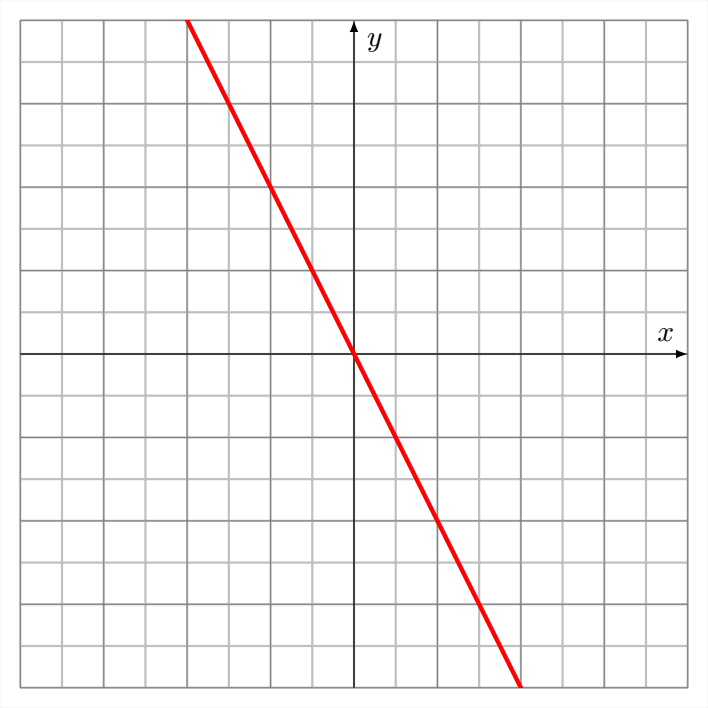
\includegraphics[width=.6\linewidth]{../images/plano_cart_rect_-2x.png}\\
				\fillin[$y=-2x$][2in]

				\part
				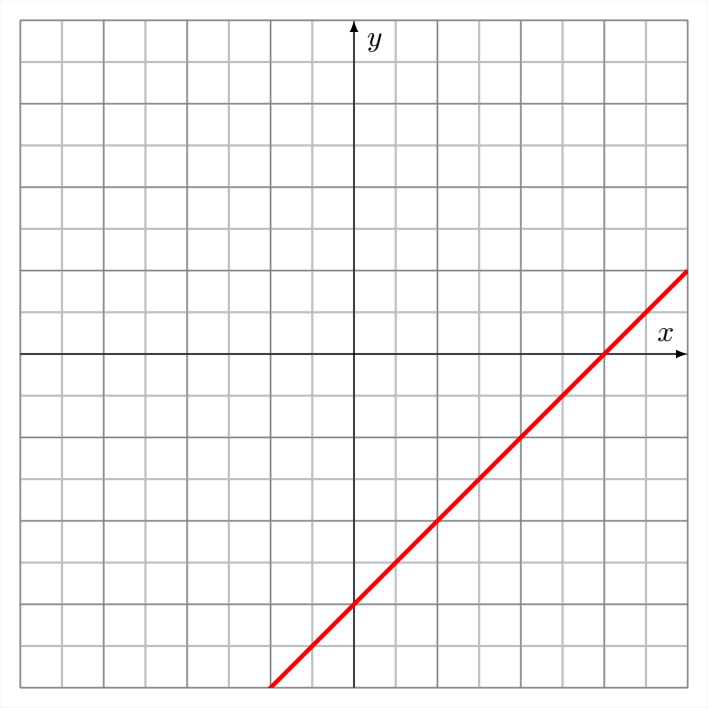
\includegraphics[width=.6\linewidth]{../images/plano_cart_rect_x-6.png}\\
				\fillin[$y=x-6$][2in]
			\end{parts}
		\end{multicols}
	}

	% \addcontentsline{toc}{section}{Porcentajes}
	\section{Porcentajes}

	% \addcontentsline{toc}{subsection}{Porcentajes a decimal}
	\subsection{Porcentajes a decimal}

	\questionboxed[2]{Escribe el número decimal que representa cada porcentaje:

		\begin{multicols}{2}
			\begin{parts}
				\part Convierte 401\% a un número decimal. \fillin[$4.01$][0in]
				\part Convierte 100\% a un número decimal. \fillin[$1$][0in]
				\part Convierte 10\% a un número decimal. \fillin[$0.1$][0in]
				\part Convierte 6\% a un número decimal. \fillin[$0.06$][0in]
				\part Convierte 0.5\% a un número decimal. \fillin[$0.005$][0in]
				\part Convierte 150\% a un número decimal. \fillin[$1.5$][0in]
				\part Convierte 33\% a un número decimal. \fillin[$0.33$][0in]
				\part Convierte 20.9\% a un número decimal. \fillin[$0.209$][0in]
				\part Convierte 3.2\% a un número decimal. \fillin[$0.032$][0in]
				\part Convierte 37.5\% a un número decimal. \fillin[$0.375$][0in]
			\end{parts}
		\end{multicols}
	}


	% \addcontentsline{toc}{subsection}{Decimal a porcentaje}
	\subsection{Decimal a porcentaje}

	\questionboxed[2]{Escribe el porcentaje que representa cada número decimal:

		\begin{multicols}{2}
			\begin{parts}
				\part Expresa 1.44 como un porcentaje. \fillin[$144\%$][0in]
				\part Expresa 1 como un porcentaje. \fillin[$100\%$][0in]
				\part Expresa 0.1 como un porcentaje. \fillin[$10\%$][0in]
				\part Expresa 2.5 como un porcentaje. \fillin[$250\%$][0in]
				\part Expresa 0.001 como un porcentaje. \fillin[$0.1\%$][0in]
				\part Expresa 0.9 como un porcentaje. \fillin[$90\%$][0in]
				\part Expresa 0.05 como un porcentaje. \fillin[$5\%$][0in]
				\part Expresa 0.33 como un porcentaje. \fillin[$33\%$][0in]
				\part Expresa 0.092 como un porcentaje. \fillin[$9.2\%$][0in]
				\part Expresa 0.209 como un porcentaje. \fillin[$20.9\%$][0in]
			\end{parts}
		\end{multicols}
	}


	% \addcontentsline{toc}{subsection}{Porcentaje de cantidades}
	\subsection{Porcentaje de cantidades}

	\questionboxed[4]{Calcula los porcentajes de cada una de las siguientes cantidades:

		\begin{multicols}{2}
			\begin{parts}
				\part ¿Cuál es el 225\% de 600?
				
				\begin{solutionbox}{1.2cm}
					\[\dfrac{600\times 225\%}{100\%}=1350\]
				\end{solutionbox}

				\part Si se sabe que 30 es el 6\% de cierta cantidad, ¿cuál es esta cantidad?
				
				\begin{solutionbox}{1.2cm}
					\[\dfrac{30\times 100\%}{6\%}=500\]
				\end{solutionbox}

				\part ¿Cuál es el 23\% de 59?
				
				\begin{solutionbox}{1.2cm}
					\[\dfrac{59\times 23\%}{100\%}=13.57\]
				\end{solutionbox}

				\part Si se sabe que 40 es el 250\% de cierta cantidad, ¿cuál es esta cantidad?
				
				\begin{solutionbox}{1.2cm}
					\[\dfrac{40\times 100\%}{250\%}=16\]
				\end{solutionbox}
			\end{parts}
		\end{multicols}
	}

	\subsection{Resolución de problemas}

	\questionboxed[10]{Resuelve los siguientes problemas:

		\begin{parts}
			\part El costo de una camisa es de \$800 pesos, si se les hace un descuento del 20\%, ¿cuánto pagaré en total por la camisa?
			
			\begin{solutionbox}{1.5cm}
				\[\$800\times 20\%=\$160\]
				\[\$800-\$160=\$640\]
			\end{solutionbox}

			\part El 24\% de los habitantes de un pueblo tienen menos de 30 años. ¿Cuántos habitantes tiene el pueblo si hay 120 jóvenes menores de 30 años?
			
			\begin{solutionbox}{1.2cm}
				\[\dfrac{120\times 100\%}{24\%}=500\]
			\end{solutionbox}
		\end{parts}
	}
\end{questions}
\end{document}